\subsection{Четырёхволновое смешение}\label{subsec:fwm}
\subsubsection{Нелинейное волновое уравнение}

Четырёхволновое смешение (ЧВС) относится к параметрическим процессам третьего порядка, при которых три фотона передают свою энергию одному фотону на суммарной частоте либо два фотона аннигилируют с рождением двух новых фотонов при сохранении энергии и импульса \cite{agrawal2019} (см. схему на рис.~\cref{fig:fwm_principle}). Процесс с участием трёх фотонов, включающий в себя, в частности, генерацию третьей гармоники, требует выполнения крайне жёстких условий фазового синхронизма и в ОВ реализуется с низкой эффективностью, поэтому в дальнейшем рассматриваться не будет. В отличие от вынужденного рассеяния (ВКР или ВРМБ), где условие фазового синхронизма выполняется автоматически за счёт изменения свойств самой среды, при ЧВС необходимо целенаправленно обеспечивать фазовый синхронизм между взаимодействующими волнами путём выбора частот накачки и параметров волокна. Для вывода связанных уравнений, описывающих эволюцию комплексных амплитуд четырёх волн при ЧВС в оптическом волокне, принимаются следующие исходные положения:

\begin{figure}[htbp]
	\centering
	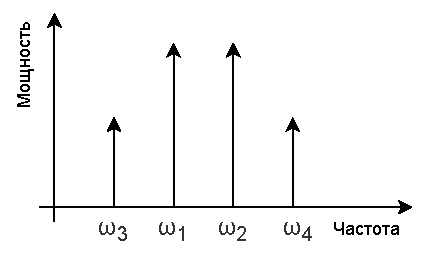
\includegraphics[width=0.4\linewidth]{Dissertation/images/review/fwm_principle}
	\caption{Принципиальная схема процесса ЧВС. Из закона сохранения энергии следует, что $\omega_1+\omega_2=\omega_3+\omega_4$}
	\label{fig:fwm_principle}
\end{figure}


\nomenclature{CW}{Сontinuous wave}
\nomenclature{QCW}{Quasi-continuous wave}


\begin{enumerate}
	\item Начинаем рассмотрение с волнового уравнения~\cref{eq:wave}, в котором нелинейная поляризация среды определяется откликом третьего порядка:
	\begin{equation*}
		\mathbf{P}_{\text{NL}} = \varepsilon_0 \chi^{(3)} \vdots \mathbf{EEE}
	\end{equation*}
	
	\item Рассматриваем скалярное приближение: все четыре взаимодействующие волны линейно поляризованы вдоль одной из осей, что обеспечивается использованием волокон с сохранением поляризации (например, типа PANDA)~\cite{fud3562,fud3564}. Данное приближение позволяет перейти от векторного описания к скалярному.
	
	\item Считаем излучение считается непрерывным (CW) или квазинепрерывным (QCW), что позволяет пренебречь зависимостью комплексных огибающих от времени. Данное приближение справедливо, если длительность оптического импульса значительно превышает как время нелинейного отклика среды (в кварцевом стекле составляет порядка нескольких фемтосекунд), так и масштаб дисперсионного уширения импульсов на длине волокна. В данной работе используются импульсы длительностью 2~нс, что удовлетворяет указанным критериям.
	
	\item Полагаем, что каждой спектральной компоненте соответствует своя поперечная мода ОВ, что учитывается при интегрировании по сечению и введении эффективной площади моды. Пространственная зависимость спектральных компонент представляется в виде
	\begin{equation*}
		E_j(\mathbf{r}) = F_j(x,y) A_j(z),
	\end{equation*}
	где $F_j(x,y)$~--- пространственное распределение $j$-й спектральной компоненты в поперечном сечении волокна.
\end{enumerate}


\begin{equation}
	\left\{\begin{array}{@{}l@{}}
		\dfrac{dA_1}{dz}=\dfrac{\im n_{nl} \omega_1}{c}\!\left[\left(f_{11}\left|A_1\right|^2+\sum\limits_{k\neq1}f_{1k}\left|A_k\right|^2\right)\!A_1+2f_{1234}A_2^{\ast}A_3A_4\e^{\im \Delta k z}\right]\!, \vspace{0.05cm} \\ 
		\dfrac{dA_2}{dz}=\dfrac{\im n_{nl} \omega_2}{c}\!\left[\left(f_{22}\left|A_2\right|^2+\sum\limits_{k\neq2}f_{2k}\left|A_k\right|^2\right)\!A_2+2f_{2134}A_1^{\ast}A_3A_4\e^{\im \Delta k z}\right], \vspace{0.05cm} \\
		\dfrac{dA_3}{dz}=\dfrac{\im n_{nl} \omega_3}{c}\!\left[\left(f_{33}\left|A_3\right|^2+\sum\limits_{k\neq3}f_{3k}\left|A_k\right|^2\right)\!A_3+2f_{3412}A_4^{\ast}A_2A_1\e^{-\im \Delta k z}\right], \vspace{0.05cm} \\
		\dfrac{dA_4}{dz}=\dfrac{\im n_{nl} \omega_4}{c}\!\left[\left(f_{44}\left|A_4\right|^2+\sum\limits_{k\neq4}f_{4k}\left|A_k\right|^2\right)\!A_4+2f_{4312}A_3^{\ast}A_2A_1\e^{-\im \Delta k z}\right].
	\end{array}\right.\,	
	\label{eq:mainEQfwm}
\end{equation}

Здесь $A_{{i}}$~--- амплитуды взаимодействующих волн с циклическими частотами $\omega_i$; $n_{nl}$~--- нелинейный показатель преломления; $f_{ij}\text{ и }f_{ijkl}$ $\left(i,j,k,l\in\left[1,\,4\right]\right)$~--- интегралы перекрытия между поперечными модами ОВ и их парами соответственно; $z$~--- продольная координата; $\Delta k$~--- волновая расстройка:


\begin{equation}
	\Delta k ={{n_3}\omega_3}/{c}+{{n_4}\omega_4}/{c}-{{n_1}\omega_1}/{c}-{{n_2}\omega_2}/{c}.
	\label{eq:deltaK}
\end{equation}

Здесь ${n_{i}}$~--- эффективный модовый показатель преломления, $c$~--- скорость света в вакууме.

Система уравнений~\cref{eq:mainEQfwm} допускает аналитическое решение в приближении неистощимой накачки. В рамках этого приближения амплитуды волн накачки считаются постоянными по длине волокна: \(|A_1(z)| \approx \mathrm{const}\) и \(|A_2(z)| \approx \mathrm{const}\).

Будем считать интегралы перекрытия приблизительно равными и обратно пропорциональными эффективной площади моды \(A_{\text{eff}}\):

\begin{equation}
	f_{ij} \approx f_{ijkl} \approx 1/A_{\text{eff}},\quad \left(i,j,k,l=1,2,3,4 \right),
	\label{eq:f_ij_ijkl_same}
\end{equation}

В этом случае эволюция сигнальной и холостой волн определяется величиной обобщённой фазовой расстройки $\kappa$:

\begin{equation}
	\kappa \coloneqq \Delta k  + \gamma\left(P_1 + P_2\right)
	\label{eq:nondepleted_phase_sync}
\end{equation}

где \(P_1 = |A_1|^2\) и \(P_2 = |A_2|^2\)~--- мощности волн накачки, \(\Delta k\) определяется выражением~\cref{eq:deltaK}, \(\gamma_i = n_2 \omega_i / (c A_{\text{eff}})\approx \gamma\).

При условии $\kappa=0$ зависимость мощности сигнальной и холостой волн от продольной координаты \(z\) становится экспоненциальной. Зависимость коэффициента усиления $g$ от величины обобщённой фазовой расстройки имеет вид:

\begin{equation}
	g=\sqrt{\left(2\gamma\sqrt{P_1 P_2}\right)^2-\left(\kappa/2\right)^2}
	\label{eq:gain_fwm}
\end{equation}

Оценки показывают~\cite{agrawal2019}, что коэффициент параметрического усиления при ЧВС превышает пиковое значение рамановского усиления примерно на $70\%$. Как следствие, при обеспечении условий фазового синхронизма порог возникновения ЧВС оказывается  ниже порога ВКР.

Взаимное влияние ЧВС и ВКР может приводить к интересным с научной точки зрения и полезным с практической точки зрения результатам. Так, в работе~\cite{eibl2017pulse} экспериментально продемонстрирована возможность создания трёхволнового лазерного источника на основе механизма комбинационного смещения с параметрической затравкой. В работе используется стандартное одномодовое волокно с положительной дисперией.  В такой среде условия фазового синхронизма для ЧВС не выполняются, и генерация новых спектральных компонент за счет только этого процесса была бы подавлена. Принципиальная схема установки приведена на рис.~\ref{fig:fewe_fwm}.
\nomenclature{MOPA}{Master Oscillator Fiber Amplifier}
\nomenclature{EOM}{Electro-Optic Modulator}
\nomenclature{YDFA}{Ytterbium Doped Fiber Amplifier}
\nomenclature{WDM}{Wavelength Division Multiplexer}
\nomenclature{OSA}{Optical Spectrum Analyzer}


\begin{figure}[htbp]
	\centering
	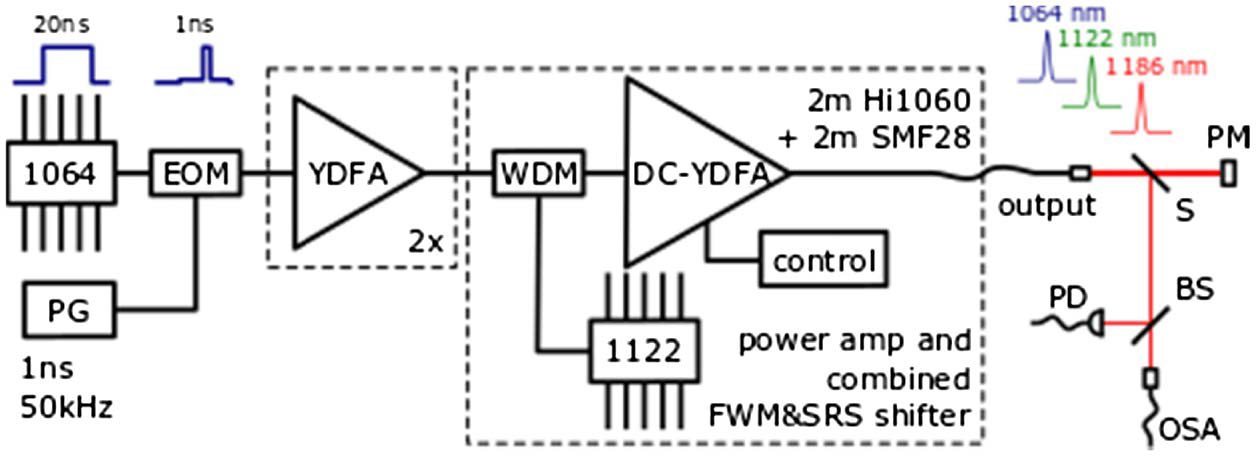
\includegraphics[width=0.6\linewidth]{Dissertation/images/review/fewe_scheme}
	\caption{Схема эксперимента. EOM~--- электрооптический модулятор; YDFA~--- иттербиевый волоконный усилитель; WDM~--- мультиплексор; OSA~--- оптический спектроанализатор.}
	\label{fig:fewe_scheme}
\end{figure}

Установка, изображённая на рис.~\cref{fig:fewe_scheme}, включает иттербиевый волоконный усилитель, работающий по MOPA-схеме и генерирующий импульсы накачки на $1064$~нм, а также задающий лазерный диод, обеспечивающий слабую затравочную волну на $1122$~нм, соответствующую первому стоксовому сдвигу.

При пиковой мощности накачки менее $1$~кВт на выходе преобладает излучение на длине волны $1064$~нм. С повышением мощности до величины около $1.3$~кВт вследствие развития эффекта ВКР усиливается и становится доминирующей спектральная компонента на $1122$~нм. При дальнейшем увеличении оптической мощности вступает в силу совместное действие каскадного ВКР и ЧВС, в котором волна $1122$~нм выступает в роли накачки, а волна $1186$~нм~--- в роли холостой компоненты. Поскольку её частота попадает в полосу стоксового усиления, повышение её мощности возможно даже в отсутствие фазового синхронизма для ЧВС. Высокий коэффициент усиления достигается за счет ВКР, а узкая спектральная линия формируется благодаря параметрической природе ЧВС-затравки. Описанная динамика переключения длин волн проиллюстрирована на рис.~\cref{fig:fewe_fwm}.

\begin{figure}[htbp]
	\centering
	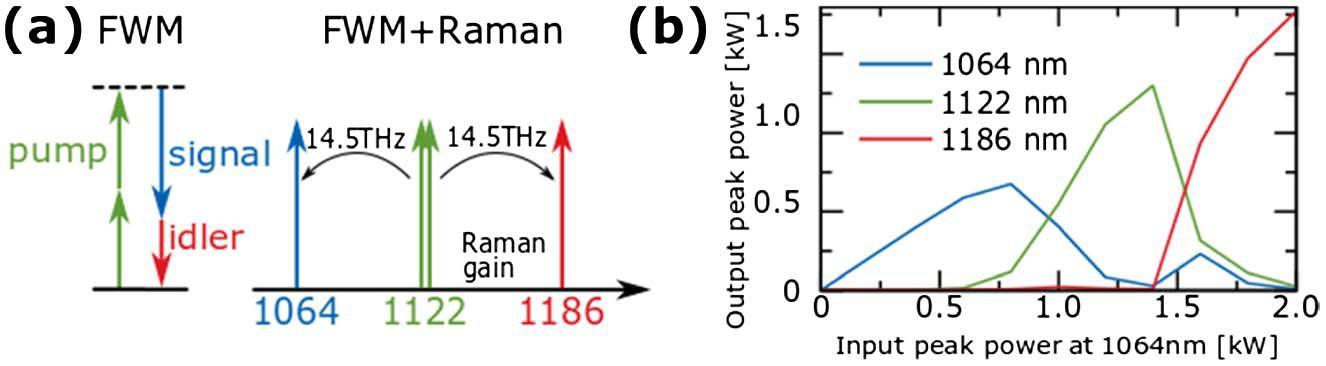
\includegraphics[width=0.7\linewidth]{Dissertation/images/review/fewe_fwm}
	\caption{(а) Совместное действие ЧВС и ВКР в ОВ приводит к генерации узкополосного излучения на $1186$~нм. (б) Результаты моделирования выходной мощности для трёх спектральных компонент ($1064$, $1122$ и $1186$~нм) при изменении мощности накачки на $1064$~нм и фиксированной мощности затравки на $1122$~нм}
	\label{fig:fewe_fwm}
\end{figure}

 Результаты данной работы показывают, что взаимное влияние двух н-о процессов могут приводить эффективной генерации новых спектральных компонент даже в отсутствие фазового синхронизма. Тем не менее, в практических применениях, когда эффект ВКР проявляется в меньшей степени, эффективность ЧВС критически зависит именно от выполнения условий фазового синхронизма. В связи с этим далее рассматриваются физические механизмы и практические методы его обеспечения.

\subsubsection{Фазовый синхронизм при ЧВС}
\subsubsection{Подавление ММЧВС}